\documentclass[14pt]{extarticle}
\usepackage[margin=1in]{geometry}
\usepackage{hyperref,xcolor,graphicx,wrapfig,lipsum}
\definecolor{crimson}{rgb}{0.86, 0.08, 0.24}
\hypersetup{
    colorlinks=true,
    linkcolor=crimson,
    filecolor=crimson,      
    urlcolor=crimson,
    citecolor=crimson,
}
\urlstyle{same}

\begin{document}
This week, we had two main goals. First, we wanted to model our data from last week to interpolate the data, calculate a $Q$ score for our first pipe, and then interpret this calculation to determine if our experimental process is sensible. Then, we sought to work on developing an automatic data collection process of some form to reduce uncertainty and annoyance throughout the collection process (perhaps through using the oscilloscope). The first task was fairly successful, and through it, I determined that my original analytical function for modelling the data,
\begin{equation}
A(f) = \frac{A_0}{\sqrt{(f_0^2 - f^2)^2 + (2\gamma f)^2}} + C
\end{equation}
is actually incorrect, because at resonance, the amplitude becomes
\begin{equation}
  A(f_0) = \frac{A_0}{2\gamma f_0} + C,
\end{equation}
thus, to make the amplitude the desired $A_0 + C$, I have to switch the functional form to
\begin{equation}
  A(f) = \frac{A_0 2 \gamma f_0}{\sqrt{(f_0^2 - f^2)^2 + (2\gamma f)^2}} + C,
\end{equation}
so through this week's work, I was able to find an analytical function for interpolating the frequency domain data that makes sense. This was especially proven through directly modelling the data, which yielded the figure below.

\begin{wrapfigure}{l}{0.6\textwidth}
  \centering
  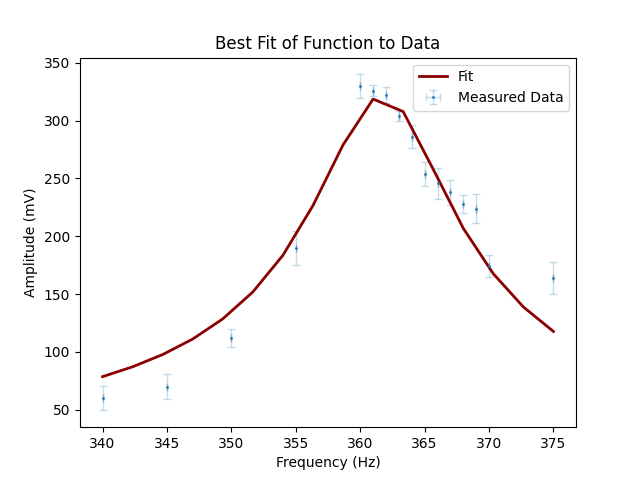
\includegraphics[width=0.6\textwidth]{autofit-graph.png}
\end{wrapfigure}

The plot yielded $\chi^2 = 5.447$, so the model is by no means a perfect fit, but this is likely good enough for reasonably estimating $Q$. The problem with this, however, is that this necessitates a precise calculation of the uncertainty in $Q$, and right now, this curve fitting process is heavily underestimating the uncertainty in its parameters, perhaps as the result of an underestimated uncertainty in the data points or computational error in the fitting process. Using the model parameters, I calculated an acoustic $Q$ of
\begin{equation}
  Q \simeq 34.03304 \pm 0.0050
\end{equation}
which is an incredibly low relative uncertainty (about $0.15\%$) despite my calculated $Q$ score being quite different from my partner Eric's (he calculated roughly 28 or so). This means that the primary goal for future experimentation will be to pursue highly precise estimation in uncertainty, as there is clearly a problem with my uncertainty measurement and/or propagation.

The second task we attempted was automatic data collection. This was a largely fruitless effort. We couldn't figure out how to work the Oscilloscope to setup automatic collection, as the plan would have been to enable datastreaming, but what Joss mentioned as a possibility would be to develop my own testing apparatus to compute the fourier transform on the fly. This sounds like it would be fun, as I could produce an automatic control system by directly connecting to the microphone on the apparatus and writing my own control code. I'll need to look into Fourier Transforms to develop a system for this, though.

Altogether, for next week, I'm hoping to do the following things:
\begin{enumerate}
\item I want to take a full set of frequency data using the oscilloscope (likely manually) for any two pipes of entirely varying lengths. This is to get the main purpose of this investigation out of the way to begin with, just so that we can have some data to answer our fundamental research question before optimizing our data collection and analysis pipeline.
\item I want to develop and test a system for automatic experimentation, so this means either finally figuring out how to use the oscilloscope (given additional time) or developing a custom Fourier wave analyzer on my own computer before the next lab. The reason for this is to expedite the data collection process.
\item I want to fix the uncertainty propagation/determination problem for calculating the $Q$ factor. I need to determine the source of underestimation in the uncertainty in $Q$ to have accurate results to report.
\end{enumerate}
\end{document}
